\documentclass[12pt,letterpaper]{article}

\pdfoutput=1

\usepackage[OT1]{fontenc}
\usepackage[colorlinks,citecolor=blue,urlcolor=blue]{hyperref}
\usepackage[pdftex]{graphicx}
\usepackage{subfig}
\usepackage{fullpage}
\usepackage{amsmath,mathtools}
\usepackage{amsfonts}
\usepackage{amsthm}
\usepackage{amssymb}
\usepackage{color}
\usepackage{todonotes}
\usepackage{listings}
\usepackage{framed}
\usepackage{common}
\usepackage{graphicx}
\usepackage[mmddyyyy,hhmmss]{datetime}
\newcommand{\Bern}{\operatorname{Bern}}
%\newcommand{\argmax}{\operatorname{argmax}}
\newcommand{\norm}[1]{\left\lVert#1\right\rVert}
\newcommand{\BR}{\mathbb R}

\newtheorem{exercise}{Exercise}

\newboolean{solutionCopy}
\setboolean{solutionCopy}{true} 

\ifthenelse{\boolean{solutionCopy}}{
  \includeversion{solution}
}{
  \excludeversion{solution}
}

\newenvironment{exercisesolution}
  {\begin{proof}[Solution]}
  {\end{proof}}
\begin{document}

\ifthenelse{\boolean{solutionCopy}}{
    \begin{center}
        {\LARGE CS 181 Spring 2022 Section 9\\
            GMMs, LDA, pLSA\\
            }
    \end{center}
}{
    \begin{center}
        {\LARGE CS 181 Spring 2022 Section 9}\\
        HMMs, Kalman Filters, and MDP's
    \end{center}
}

\section{Mixture Models}

\subsection{Motivation}


A \textit{mixture model} is a type of probabilistic
model for unsupervised learning. Suppose you have some observed data $\{ \boldx_n \}_{n = 1}^{N}$.  Mixture models are used when you have reason to believe that each individual observation has a discrete \textit{latent variable} $\boldz_n$ that determines the data generating process. A latent variable is some piece of data that is unknown, but influences the observed data.

Say there are $K$ possible values for each $\boldz_n$, denoted $\{C_k\}_{k=1}^K$ where each $C_k$ is a one-hot encoded vector of length $K$. 

Consider the following data-generating process for each data point $\boldx_n$:

\begin{itemize} 
    \item Sample latent class $\boldz_n$ from $\btheta$, the categorical distribution over $\{C_k\}_{k=1}^K$ s.t. \\$p(\boldz = C_k; \btheta) = \theta_k$.  Call this sampled latent class $C_S$.
    \item Given that $\boldz_n = C_S$, sample $\boldx_n$ from the distribution
    $$p(\boldx | \boldz = C_S; \boldw)$$
    
    This conditional distribution is a modeling assumption (which means we will give it to you in this class), and is specified using unknown parameters $\boldw$.
    
    For example, we may assume that $\boldx \sim p(\boldx | \boldz = C_k) = \mathcal{N}(\boldx; \bmu_k, \bSigma_k)$, where $\bmu_k, \bSigma_k$ are the unknown mean and covariance of the $k$-th cluster.  (See Section 2.4 for more about Gaussian mixture models!)
\end{itemize}

\emph{Example:}  Say you have a dataset containing weights from a random sample of animals in a pet store.  Each $x_n$ is the animal's weight.  The latent variables $z_n$ represent what kind of animal is being weighed, so the possible values $\{C_1, C_2, \ldots, C_K\}$ may represent the categories cat, dog, bird, etc.  In your model, you also use the assumption that $p(x | z = C_k ; \boldw) \sim N(\mu_k, \sigma_k)$.

\vspace{2em}
\begin{exercise}
In this example, can you give an intuitive explanation of what vector $\btheta$ represents?  What does it mean that $p(x | z = C_k ; \boldw) \sim N(\mu_k, \sigma_k)$?
\end{exercise}

\begin{solution}
    \begin{exercisesolution}
    $\btheta$ represents the proportion of each type of animal in the pet store.  For example, if $\theta_k = 0.2$ and $C_k$ represents dogs, then 20\% of all animals in the pet stores are dogs (or, if an animal is chosen at random, there is a 20\% chance it will be a dog).

    This class-conditional distribution means that for each type of animal, the weights of the animal are distributed normally with a fixed mean and variance for that animal.  
    \end{exercisesolution}
\end{solution}


% \begin{exercise}
% concept question from 5 minute stats related to why we can't just add the two normals, 
% \url{https://stephens999.github.io/fiveMinuteStats/intro_to_mixture_models.html}
% \end{exercise}
% \begin{solution}
% \begin{exercisesolution}
    
% \end{exercisesolution}
% \end{solution}

\section{Expectation Maximization Recap}

Expectation maximization is a general technique for maximum-likelihood estimation used primarily for models with latent variables. Here we will show how to use EM to train a mixture model, but EM is also used for a variety of other models!

\smallskip 

Consider a generative mixture model consisting of a latent variable $\boldz$ from a distribution $p(\boldz; \btheta)$ and an observed variable $\boldx$, such that we draw $\boldx$ from a distribution $p(\boldx | \boldz; \boldw)$.

\smallskip

We have 2 goals: 

\begin{itemize}
    \item[1.] To compute the MLE for $\boldw$ and $\btheta$, i.e. the values of $\boldw$, $\btheta$ that maximize $p(\boldx; \boldw, \btheta)$.
    \item[2.] To estimate the latent variable $\boldz_n$ corresponding to a particular $\boldx_n$, which in this case means maximize the distribution $p(\boldz_n | \boldx_n; \boldw, \btheta)$.
\end{itemize}

Goal 2 is easy once we have an estimate of the MLE for $\boldw, \btheta$, because we can apply Bayes' rule:
$$p(\boldz | \boldx; \boldw, \btheta) \propto p(\boldx | \boldz; \boldw, \btheta )p(\boldz; \boldw, \btheta)$$
\begin{align}p(\boldz | \boldx; \boldw, \btheta) \propto p(\boldx | \boldz; \boldw)p(\boldz; \btheta)\end{align}

\subsection{Why EM?}
The likelihood of the data can be written as 

$$p(\boldx; \boldw, \btheta) = \sum_{\boldz \in Z} p(\boldx, \boldz; \boldw, \btheta)$$

Unfortunately calculating the MLE is often computationally intractable, because the log-likelihood is:
\begin{align}
    \log p(\boldx; \boldw, \btheta) = \log \sum_{\boldz \in Z} p(\boldx, \boldz; \boldw, \btheta)
\end{align}

There is no closed form for the MLE of the log-likelihood because it is the log of a sum of expressions.  We know the form of the model $p(\boldx, \boldz; \boldw, \btheta)$, but in general we cannot solve for the $(\boldw, \btheta)$ which maximize the likelihood $p(\boldx; \boldw, \btheta)$ in closed form. 

\newpage
\subsection{The EM Algorithm}


Since finding the MLE directly is difficult, we will use expectation maximization: an approximate iterative approach. The steps of the algorithm are:

\begin{enumerate}
    \item Initialize $\boldw^{(0)}, \btheta^{(0)}$ randomly.
    \item \textit{(E-step)} Use the parameters to predict the distribution $\boldq$ for each example. The vector $\boldq_n$ represents how likely it is that the latent variable $\boldz_n$ comes from each class, given our current setting for the model parameters:
    \begin{align} q_{n,k} := p(\boldz_n = C_k | \boldx_n; \boldw^{(t)}, \btheta^{(t)}) \propto p(\boldx_n | \boldz_n=C_k; \boldw^{(t)})p(\boldz_n=C_k; \btheta^{(t)})\end{align}
    \item \textit{(M-step)} Update parameters: Choose the value of $\boldw^{(t + 1)}, \btheta^{(t + 1)}$ that maximizes the expected complete data log likelihood (where the expectation is over the distribution calculated above):
    \begin{align}
    \boldw^{(t + 1)}, \btheta^{(t + 1)} = \underset{\boldw, \btheta}\argmax\: \mathbb{E}_{\boldZ | \boldX}\left[\sum_{n=1}^N \log p(\boldx, \boldz; \boldw, \btheta)\right]
    \end{align}
    \item Go back to step 2 until the log-likelihood estimate in step 3 converges.
\end{enumerate}


\section{Dice Example: Mixture of Multinomials}
\label{dice}
    
    Consider the following example scenario: we have two biased dice (with 6 faces) and one biased coin (with 2 sides). Data is generated as follows: first, the biased coin is flipped. Suppose it lands heads. Then dice 1 is rolled $c=10$ times. This gives the first example, i.e., $\mathbf{x}_1$ would correspond to the number of times of rolling each of a $1, 2, \ldots, 6$. Then we repeat, flipping the biased coin. Suppose it lands tails. Then Dice 2 is rolled 10 times. We record the result of the dice rolls as $\mathbf{x}_2$. We keep repeating, obtaining additional examples. 

   For example, our observations for the first 10 rolls may look like: 
    $    1, 5, 3, 4, 2, 2, 3, 1, 6, 2$ and we'd record as our first example
\begin{align*}
    \textbf{x}_1 =
        \begin{bmatrix}
            2 \\
            3 \\
            2 \\
            1 \\
            1 \\
            1
        \end{bmatrix} 
\end{align*}


We're going to try to infer the parameters of each of the dice based on these observations.
%
Let's consider how this scenario fits into our idea of a mixture model. First, the latent variable $\textbf{z}_n$ has a natural interpretation as being which dice was rolled for the $n^{th}$ observed data point $\textbf{x}_n$. We can represent $\textbf{z}_n$ using a one-hot vector, so that if the $n^{th}$ data point came from Dice 1, we'd denote that:
\begin{align*}
    \textbf{z}_n =
        \begin{bmatrix}
            1 \\
            0 \\
        \end{bmatrix} \\
\end{align*}

We denote the probability vector associated with the biased coin as $\boldsymbol{\theta} \in [0,1]^{2}$, summing to 1, with $\theta_1$ being the probability of the biased coin landing heads and $\theta_2$ being the probability of the biased coin landing tails. Furthermore, we need parameters to describe the behavior of the biased dice. We use $\boldsymbol{\pi_1}, \boldsymbol{\pi}_2 \in [0,1]^{6}$, summing to 1, where each 6-dimensional vector describes the probability that the respective dice lands on each face.

For a given dice, this defines a multinomial distribution. For $c$ trials, and counts $x_1, \ldots, x_6$ for each of 6 faces on a 6-sided dice, and probabilities $\boldsymbol{\pi}$, this is
%
\begin{align}
  p(\mathbf{x}; \boldsymbol{\pi})&=\frac{c!}{x_1!\cdot \ldots \cdot x_6!}\pi_1^{x_1}\cdot \ldots \cdot \pi_6^{x_6}
\end{align}

For our purposes, let $ p(\textbf{x}_n | \textbf{z}_n = C_k; \boldsymbol{\pi}_1, \boldsymbol{\pi}_2)$ denote the
multinomial distribution on observation $\textbf{x}_{nj}$ when latent vector $\textbf{z}_n = C_k$.

%
%
The model parameters are $\textbf{w} = \{\boldsymbol{\theta}, \boldsymbol{\pi}_1, \boldsymbol{\pi}_2 \}$.
We can optimize the model parameters using EM. We start by initializing the parameters $\boldsymbol{\theta}^{(0)}, \boldsymbol{\pi}^{(0)}$.

In the E-step, we compute the soft assignment values, $\textbf{q}_n$. For dice $k$, this given by
%
\begin{align} \label{E-for-multinomial}
q_{nk} = 
&  p(\textbf{z}_n = C_k | \textbf{x}_n; \boldsymbol{\theta}^{(i)}, \boldsymbol{\pi}^{(i)})
\\
&  =
     \frac{  p(\textbf{x}_n | \textbf{z}_n = C_k; \boldsymbol{\pi}^{(i)})p(\textbf{z}_n = C_k; \boldsymbol{\theta}^{(i)})}
     {\sum_{k=1}^K  p(\textbf{x}_n | \textbf{z}_n = C_k; \boldsymbol{\pi}^{(i)})p(\textbf{z}_n = C_k; \boldsymbol{\theta}^{(i)})}
  \\
  &  =
     \frac{  p(\textbf{x}_n | \textbf{z}_n = C_k; \boldsymbol{\pi}^{(i)})\theta_k^{(i)}}
     {\sum_{k=1}^K  p(\textbf{x}_n | \textbf{z}_n = C_k; \boldsymbol{\pi}^{(i)})\theta_k^{(i)}}
\end{align}


We could also use the ``product trick'' to write a single expression
%
\begin{align*}
  p(\textbf{z}_n  | \textbf{x}_n; \boldsymbol{\theta}^{(i)}, \boldsymbol{\pi}^{(i)})& =
 \frac{  \prod_{k=1}^K\left(  p(\textbf{x}_n | \textbf{z}_n = C_k; \boldsymbol{\pi}^{(i)})\theta_k^{(i)}\right) ^{z_{nk}}}
{\sum_{k=1}^K  p(\textbf{x}_n | \textbf{z}_n = C_k; \boldsymbol{\pi}^{(i)})\theta_k^{(i)}}
  \\
  & =
 \frac{  \prod_{k=1}^K p(\textbf{x}_n | \textbf{z}_n = C_k; \boldsymbol{\pi}^{(i)})^{z_{nk}}\prod_{k=1}^K(\theta_k^{(i)})^{z_{nk}}}
{\sum_{k=1}^K  p(\textbf{x}_n | \textbf{z}_n = C_k; \boldsymbol{\pi}^{(i)})\theta_k^{(i)}}
  \end{align*}

The vector $\textbf{q}_n$  is defined as:
%
\begin{align}
  \label{E-for-multinomial}
    \textbf{q}_n &= \begin{bmatrix}
                p(\textbf{z}_n = C_1 | \textbf{x}_n; \boldsymbol{\theta}^{(i)}, \boldsymbol{\pi}^{(i)}) \\
                p(\textbf{z}_n = C_2 | \textbf{x}_n; \boldsymbol{\theta}^{(i)}, \boldsymbol{\pi}^{(i)}) 
            \end{bmatrix} 
\end{align}


After computing the values of $\textbf{q}_n$, we are ready to perform the M-step.
Recall that we are maximizing the expected complete-data log likelihood, which takes the form:
%
\begin{align} \label{M-for-multinomial}
    \mathbb{E}_{\textbf{Z}|\textbf{X}}[\log p(\textbf{X}, \textbf{Z})] &= \mathbb{E}_{\textbf{q}_n} \bigg[\sum_{n=1}^{N} \log p(\textbf{z}_n; \boldsymbol{\theta}^{(i+1)}, \boldsymbol{\pi}^{(i+1)}) + \log p(\textbf{x}_n | \textbf{z}_n; \boldsymbol{\theta}^{(i+1)}, \boldsymbol{\pi}^{(i+1)})\bigg] \\ 
                                                                       &= \sum_{n=1}^{N} \mathbb{E}_{\textbf{z}_n|\textbf{x}_n} \bigg[ \log p(\textbf{z}_n; \boldsymbol{\theta}^{(i+1)}, \boldsymbol{\pi}^{(i+1)}) + \log p(\textbf{x}_n | \textbf{z}_n; \boldsymbol{\theta}^{(i+1)}, \boldsymbol{\pi}^{(i+1)})\bigg]
\end{align}

We can then substitute in for the multinomial expression and simplify,
and dropping constants we have that we're looking for
parameters that solve
%
\begin{align}
&  \arg\max_{\boldsymbol{\theta}^{(i+1)}, \boldsymbol{\pi}^{(i+1)}}\left\{
                \sum_{n=1}^{N} \sum_{k=1}^{2} q_{n, k}  \log \theta_k^{(i+1)} +
  \sum_{n=1}^{N} \sum_{k=1}^{2}q_{n,k}\log\left(\pi_{k,1}^{x_n,1}\cdot\ldots\cdot\pi_{k,6}^{x_n,6}\right) \right\}
 \notag \\
  &=  \arg\max_{\boldsymbol{\theta}^{(i+1)}, \boldsymbol{\pi}^{(i+1)}}\left\{
                \sum_{n=1}^{N} \sum_{k=1}^{2} q_{n, k}  \log \theta_k^{(i+1)} +
    \sum_{n=1}^{N} \sum_{k=1}^{2}\sum_{j=1}^6 q_{n,k}x_{n,j}\log(\pi_{k,j})\right\}
    \label{eq:dpnew1}
\end{align}

To maximize the expected complete-data log likelihood, it's necessary to introduce Lagrange multipliers to enforce the constraints $\sum_{k} \theta_k^{(i+1)} = 1$ and $\sum_{j} \pi_{k, j}^{(i+1)} = 1$, for each $k$. After doing this,
and solving, we recover the following update equations for the model parameters:
%
\begin{align*}
    \theta_{k}^{(i+1)} \leftarrow \frac{\sum_{n=1}^{N} q_{n, k}}{N}
\end{align*}
\begin{align*}
    \boldsymbol{\pi}_{k}^{(i+1)} \leftarrow \frac{\sum_{n=1}^{N} q_{n, k} \textbf{x}_{n}}{c \sum_{n=1}^{N} q_{n, k} },
\end{align*}
%
where $c=10$ in out example.

We now have everything we need to perform EM for this setup. After initializing our parameters $\textbf{w}^{(0)}$, we perform the E-step by evaluating \ref{E-for-multinomial}. After calculating our values of $\textbf{q}_n$ in the E-step, we update our parameters $\textbf{w} = \{\boldsymbol{\theta}, \boldsymbol{\pi}_1, \boldsymbol{\pi}_2 \}$ in the M-step by maximizing \ref{eq:dpnew1} with respect to $\boldsymbol{\theta}, \boldsymbol{\pi}_1, \boldsymbol{\pi}_2$. We perform these two steps iteratively, until convergence of our parameters.

\section{Gaussian Mixture Modeling}

%We have data $\boldx_n \in \mathbb{R}^{D}$ and a latent variable $\boldz_n$ (corresponding to the cluster that the point is drawn from) such that $\boldx \sim p(\boldx | \boldz = C_k) = \mathcal{N}(\boldx; \bmu_k, \bSigma_k)$, where $\bmu_k, \bSigma_k$ are the mean and covariance of the $k$-th cluster. The choice of cluster is drawn from a categorical distribution with probabilities $\bpi \in [0, 1]^K$. We are able to observe the data $\boldx_n$ and want to find the cluster centers and their covariances.

%The steps of EM inference applied to this problem are:
%\begin{enumerate}
%    \item Randomly initialize $\bpi, \{\bmu_k, \bSigma_k\}_{k=1}^K$.
%    \item Next, calculate the new distribution of each $\boldz_n$:
%        \begin{align}
%            q_{n,k} = p(z_n = C_k | \boldx_n) \propto \pi_k \mathcal{N}(\boldx_n; \bmu_k, \bSigma_k)
%        \end{align}
%    This is our new estimate of the distribution of $\boldz_n$ given the data and our estimate for $\bpi, \{\bmu_k, \bSigma_k\}_k$.
%    \item Find the expected complete data log-likelihood:
%    \begin{align}
%         \mathbb{E}_{\boldZ|\boldX}\left[\mcL\right] &= \mathbb{E}_{\boldZ|\boldX}[\sum_{n = 1}^N  \ln(p(\boldx_n, \boldz_n; \bpi, \{\bmu_k, \bSigma_k\}_k))] \\
%         &= \sum_{n = 1}^N \sum_{k = 1}^K q_{n,k} \ln \pi_k + q_{n,k} \ln \mathcal{N}(\boldx_n; \bmu_k, \bSigma_k) 
%    \end{align}
%    and then optimize it for each of the parameters $\bpi, \{\bmu_k, \bSigma_k\}_{k=1}^K$. However, we need to be careful to remember constraints: since $\sum_k \pi_k = 1$, we must use Lagrange multipliers to optimize the parameters. We get the following update equations:
%    \begin{align}
%        \pi_k^{(t + 1)} &= \frac{\sum_{n = 1}^N  q_{n,k}}{N} \\
%        \bmu_k^{(t + 1)} &= \frac{\sum_{n = 1}^N q_{n,k}\boldx_n}{\sum_{n = 1}^N  q_{n,k}} \\
%        \bSigma_k^{(t + 1)} &= \frac{\sum_{n = 1}^N  q_{n,k}(\boldx_n - \bmu_k^{(t + 1)})(\boldx_n - \bmu_k^{(t + 1)})^{\top}}{\sum_{n = 1}^N  q_{n,k}}
%    \end{align}
%\end{enumerate}

We now examine a commonly used 
mixture model called a Gaussian Mixture Model (GMM). As you might expect, a GMM consists of a combination of multiple Gaussian distributions. Among other things, it is useful for modeling scenarios where the observed data is continuous.

Let's go over a more rigorous formulation of the GMM setup. First, we have observed continous data $\textbf{x}_n \in \mathbb{R}^{m}$ and latent variables $\textbf{z}_n$ which indicate which Gaussian `cluster' our observed data point was drawn from. In other words:
\begin{align*}
    p(\textbf{x}_n | \textbf{z}_n = C_k) = \mathcal{N}(\textbf{x}_n; \boldsymbol{\mu}_k, \boldsymbol{\Sigma}_k)
\end{align*}
where $\boldsymbol{\mu}_k, \boldsymbol{\Sigma}_k$ are the mean and covariance parameters respectively for the $k^{th}$ cluster center.

The data generation process works as follows: we first sample a cluster center from a Categorical distribution parameterized by $\boldsymbol{\theta} \in \mathrm{R}^{K}$. Then, based on the sampled cluster center, we sample a data point $\textbf{x}_n \in \mathrm{R}^{m}$, which is the only piece of data that we actually observe. As usual for a mixture model, it is our goal to use the observed data to determine the cluster means and covariances, as well as the parameters of the Categorical distribution that selects the cluster centers.

Fortunately, this problem setup is perfectly suited for EM. We can apply the same machinery we've discussed throughout the chapter and used in the previous example.
\begin{itemize}
    \item[1.] First, we randomly initialize our parameters $\boldsymbol{\theta}, \{ \boldsymbol{\mu}_k, \boldsymbol{\Sigma}_k \}_{k=1}^{K}$.
    \item[2.] [E-Step] Calculate the posterior distribution over $\textbf{z}_n$ given by $\textbf{q}_n$:
        \begin{align*}
            \textbf{q}_n = \mathrm{E}[\textbf{z}_n | \textbf{x}_n] &= \begin{bmatrix}
                p(\textbf{z}_n = C_1 | \textbf{x}_n; \theta_1, \boldsymbol{\mu}_1, \boldsymbol{\Sigma}_1) \\
                \vdots \\
                p(\textbf{z}_n = C_K | \textbf{x}_n; \theta_K, \boldsymbol{\mu}_K, \boldsymbol{\Sigma}_K) \\
            \end{bmatrix} \\
            &\propto \begin{bmatrix}
                \theta_1 \mathcal{N}(\textbf{x}_n; \boldsymbol{\mu}_1, \boldsymbol{\Sigma}_1) \\
                \vdots \\
                \theta_K \mathcal{N}(\textbf{x}_n; \boldsymbol{\mu}_K, \boldsymbol{\Sigma}_K) \\
            \end{bmatrix} \\
        \end{align*}
        This is the current expectation for our latent variables $\textbf{z}_n$ given our data $\textbf{x}_n$ and the current setting of our model parameters $\boldsymbol{\theta}, \{ \boldsymbol{\mu}_k, \boldsymbol{\Sigma}_k \}_{k=1}^{K}$.
    \item[3.] [M-Step] Using our values of $\textbf{q}_n$, calculate the expected complete-data log likelihood, and then use that term to optimize our model parameters:
        \begin{align*}
            \mathbb{E}_{\textbf{q}_n}[\log p(\textbf{X}, \textbf{Z})] &= \mathbb{E}_{\textbf{q}_n} \bigg[ \sum_{n=1}^{N} \ln(p(\textbf{x}_n, \textbf{z}_n; \boldsymbol{\theta}, \{ \boldsymbol{\mu}_k, \boldsymbol{\Sigma}_k \}_{k=1}^{K})) \bigg] \\
            &= \sum_{n=1}^{N} \sum_{k=1}^{K} q_{n, k} \ln \theta_k + q_{n, k} \ln \mathcal{N}(\textbf{x}_n; \boldsymbol{\mu}_k, \boldsymbol{\Sigma}_k) \\
        \end{align*}
        We can then use this expected complete-data log likelihood to optimize our model parameters $\boldsymbol{\theta}, \{ \boldsymbol{\mu}_k, \boldsymbol{\Sigma}_k \}_{k=1}^{K}$ by computing the MLE as usual. Using a Lagrange multiplier to enforce $\sum_{k=1}^{K} \theta_k = 1$, we recover the update equations:
        \begin{align*}
            \theta_k^{(i + 1)} &\leftarrow \frac{\sum_{n=1}^{N} q_{n, k}}{N} \\
            \boldsymbol{\mu}_k^{(i + 1)} &\leftarrow \frac{\sum_{n=1}^{N} q_{n, k} \textbf{x}_n}{\sum_{n=1}^{N} q_{n, k}} \\
            \boldsymbol{\Sigma}_k^{(i + 1)} &\leftarrow \frac{\sum_{n=1}^{N} q_{n, k} (\textbf{x}_n - \boldsymbol{\mu}_k^{(i + 1)})(\textbf{x}_n - \boldsymbol{\mu}_k^{(i + 1)})^{T}}{\sum_{n=1}^{N} q_{n, k}} \\
        \end{align*}
    \item[4.] Return to step 2. Repeat until convergence.
\end{itemize}

\section{Topic Models}

Topic modeling is used for discovering latent topics or themes in large collections of documents. The goal is the underlying structure in a corpus of text documents and categorizing them into different groups based on their content. Topic modeling is a type of unsupervised learning, where the algorithm tries to discover patterns and structures in the data without prior knowledge of the labels or categories. Some of the popular applications of topic modeling include document clustering, text classification, and information retrieval. 

Topic modeling is similar to other latent variable models, such as Gaussian mixture models (GMMs).
%in that it involves learning the parameters of a probability distribution over a set of latent variables. However, the key difference between topic modeling and GMMs is that topic modeling assumes that the latent variables are discrete and represent topics, whereas GMMs assume that the latent variables are continuous and represent clusters. 
Like the mixture models that we study in this course, we will describe topic models generatively: one in which we assume our corpus is generated
by some process. Then, we will seek to use an optimization method, such as EM, to train the parameters of our model.

\subsection{Probabilistic Latent Semantic Analysis (pLSA)}

Consider a collection of documents, where each document is a mixture of various topics. pLSA is a generative model that assumes each word in a document is generated by sampling from a topic, and the topic is sampled from a per-document distribution. As a generative model, we want to model the joint probability of words and documents, $p(w, d)$. The generative process for a document in pLSA is as follows:
\begin{enumerate}
    \item Initialize conditional probabilities $p(z \mid d)$ and $p(w\mid z)$ that represent the per-document distribution for topics and per-topic distribution for words.
    \item For each document $d$, choose a topic $z$ with probability $p(z \mid d)$.
    \item For the chosen topic $z$, pick a word $w$ with probability $p(w \mid z)$.
\end{enumerate}

The goal of pLSA is to learn the conditional probabilities $p(w \mid z)$ and $p(z \mid d)$. In pLSA, we do not impose any priors on these probabilities beforehand. Given the observed data $p(w \mid d)$, we can train a latent model to estimate the conditional probabilities $p(w \mid z)$ and $p(z \mid d)$ based on the training data. To do this, we use the Expectation-Maximization algorithm again to maximize the likelihood of the observed data with respect to the latent variables, or the topics. The EM algorithm consists of two steps:

\begin{itemize}
    \item Expectation (E) step: Compute the posterior probabilities of the topic assignments $p(z \mid w, d)$ using the current estimates of $p(w \mid z)$ and $p(z \mid d)$. To do so, we can use the observed data likelihood function: $$p(w, d) = \sum_z p(w \mid z)p(z \mid d)p(d)$$
    \item Maximization (M) step: Update the estimates of $p(w \mid z)$ and $p(z \mid d)$ based on the posterior probabilities computed in the E step.
\end{itemize}
Note that we only know $d_j$ and $w_{ij}$ but define $z_{ij}$ in order to train the conditional probabilities in such a way that makes intuitive sense in our generative model. The plate diagram for pLSA is below:

\begin{center}
    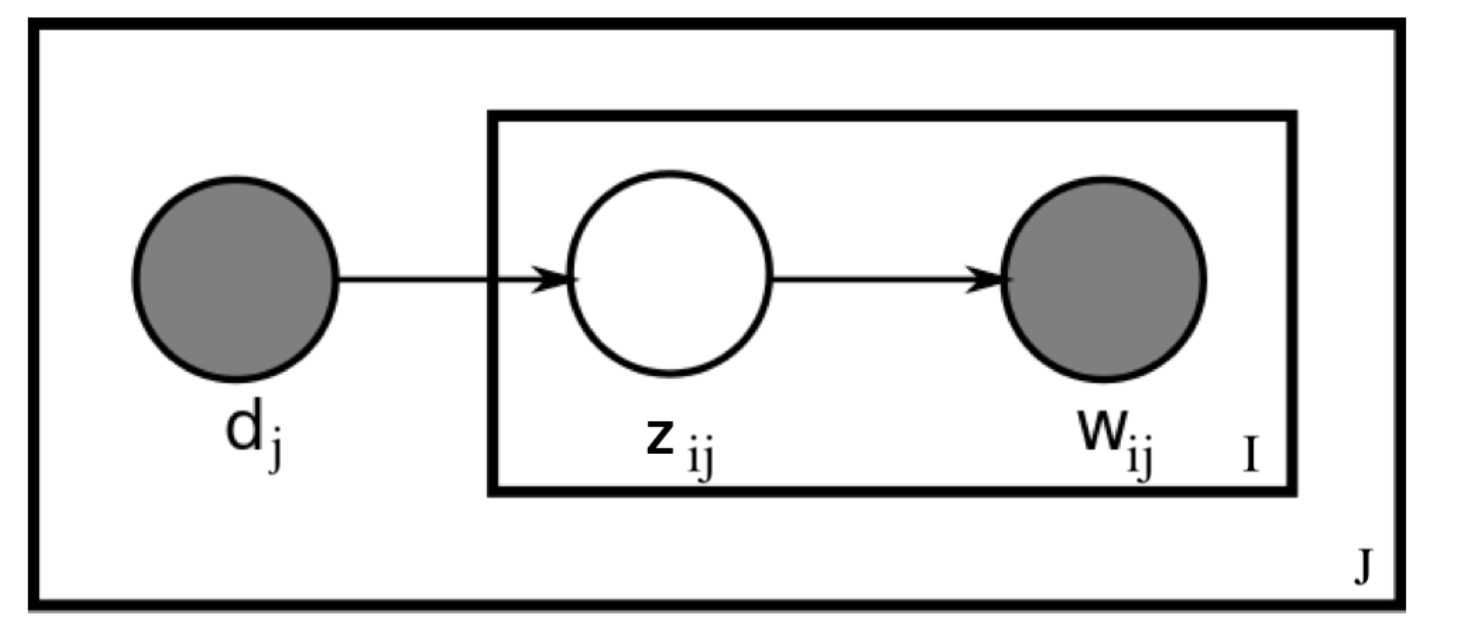
\includegraphics[scale=0.5]{pLSA.png}
\end{center}

In this relatively limited model, the most notable weakness is overfitting. As the number of parameters in the model grows linearly with the number of documents, pLSA is prone to overfitting. The model does not have a prior imposed on the per-document or per-topic distributions, so all of the parameter learning is derived from the training data. In document text, this is particularly bad because the true complexity of possible document features is far more complex than just the documents in the sample corpus.

\subsection{Latent Dirichlet Allocation (LDA)}

Latent Dirichlet Allocation (LDA) is an extension of pLSA that addresses some of its limitations, mainly overfitting and lack of a generative model for new documents. Like pLSA, LDA is a generative probabilistic model for topic modeling that assumes each document is a mixture of topics, and each topic is a distribution over words. However, LDA introduces a Dirichlet prior on the per-document topic distributions and per-topic word distributions, leading to better generalization and the ability to infer topic distributions for new documents. Specifically, we use fixed parameters $\balpha$ and $\bbeta$ as an extra ``layer'' of sampling. 

We begin by describing the generative process by which a document $i$ is generated. For topic modeling, similar to K-means, we have to begin by picking the number of topics, $K$, to look for. We define a topic $\bphi_{k}$ to be a distribution over the words, so $\bphi_{k} \in [0,1]^{|\mcW|}$, where $\mcW$ is the set of words. For each document, we have a document-topic distribution $\btheta_m \in [0,1]^K$. These are the parameters to estimate in LDA.

We now describe the data generation process:

\begin{enumerate}
    \item Let $\balpha \in \mathbb{R}_+^K$ and $\bbeta \in \mathbb{R}_+^{|\mcW|}$.
    \item For each document $m = 1, \ldots, M$, sample a mixture over topics: $\btheta_n \sim Dir(\balpha)$.
    \item For each topic $k = 1, \ldots, K$, sample a mixture over words in that topic: $\bphi_k \sim Dir(\bbeta)$.
    \item For each word $w_{m,n}$ (for $m = 1, \ldots, M$ and $n = 1, \ldots, N$, the length of the document), first sample the topic $z_{m,n} \sim Cat(\btheta_m)$, then sample the word $w_{m,n} \sim Cat(\bphi_{z_{m,n}})$.
\end{enumerate}

\noindent For some intuition, the Dirichlet distribution takes in a $k$-sized vector of values and outputs a probability distribution across $k$ categories. Roughly speaking, the Dirichlet parameter is a vector of positive real numbers; the larger the value, the more likely that corresponding component of the sampled vector will have a higher value. At a high level, then, a topic model is a mixture over mixtures: within a single document, $\btheta_m$ specifies a distribution over topics in that document, and for each topic, $k$, in that document, $\bphi_k$ specifies a distribution over words.

This process is again summarized in the following plate diagram (where $\eta$ in the diagram represents the Dirichlet parameter for words per topic):

\begin{center}
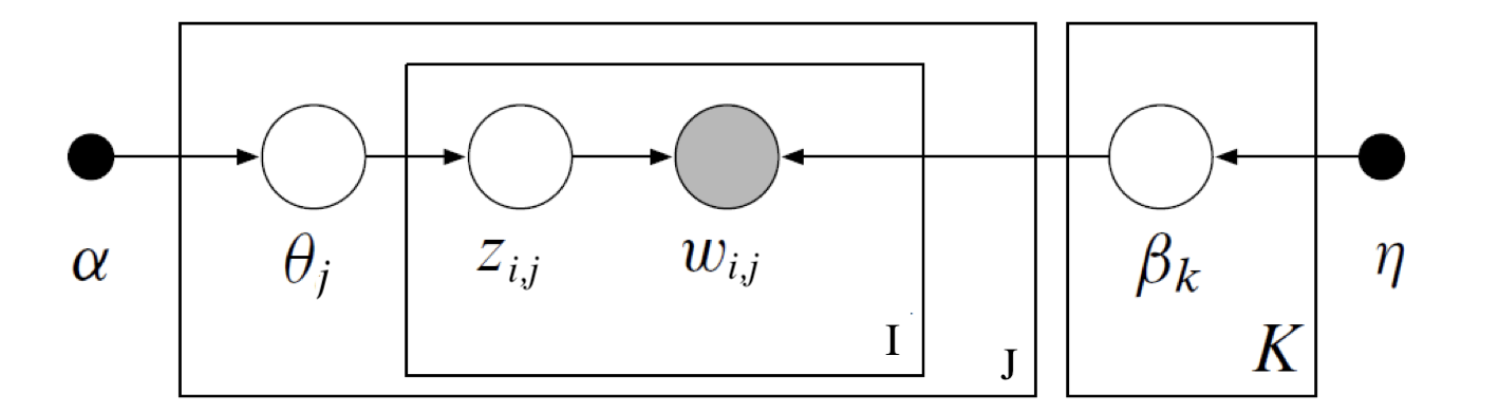
\includegraphics[scale= 0.6]{LDA.png}
\end{center}

Comparing this plate diagram to that of pLSA, we can observe that pLSA is just if we consider the plates across $I$ and $J$, without the fixed inputs of $\balpha$ and $\eta$. Like pLSA, we can use a version of EM to optimize the model parameters, but requires an approximation of the posterior distributions (variational inference).

The main takeaway from LDA is that the introduction of Dirichlet priors for the per-document topic distributions $\btheta$ and per-topic word distributions $\bphi$ acts as a form of regularization. By imposing these priors, the model incorporates some prior knowledge or assumptions about the distributions, which helps guide the learning process. This regularization effect prevents the model from relying too heavily on the training data, leading to better generalization and robustness against overfitting. As a result, LDA can more effectively estimate the underlying topic structure in the data and produce topic distributions for new, unseen documents. This makes LDA a more robust and widely applicable topic modeling method compared to pLSA, which lacks the regularization provided by the Dirichlet priors.

% \fbox{\parbox{\linewidth}{%
% \begin{exercise}
% Describe, at a high level, how the EM algorithm for topic models can be viewed as alternating between two optimizations. What are these two optimizations?
% \end{exercise}
% }}

% \begin{exercisesolution}
% In  EM, we alternate between the E step and M step. In the E step, we write the posterior distribution, $q$ of the latent variable given the data and our current estimates of the parameters, and in the M-step we try to maximize (over our parameters) the expected complete-data log likelihood under $q$. The two steps alternate between first (E step) finding a lower bound to the true log likelihood (i.e., by finding $q$ and noting that the complete-data log likelihood under $q$ minus $q$'s entropy over the dataset (which is constant w.r.t the parameters) lower bounds the true log likelihood) and then (M step) choosing the parameters which maximize this lower bound.
% \\
% \\
% In the case of topic models, we do the exact same thing. Specifically, for the $m$th document, the posterior distributions $q_{m,n}$ (which we take the expectation of the complete-data log likelihood with respect to in the M step), will be the posterior distributions of topics given words and our current estimates of the parameters. We calculate these $q_{m,n}$'s in the E step as an optimization towards establishing a lower bound on the true log likelihood, and then, in the M step, we optimize over the parameters $\btheta_m, \bphi_k$ to maximize this lower bound. Specifically, in the M step, we find parameters that maximize the expected complete-data log likelihood under $q_m$: $\mathbb{E}_{q_m}[\log p(\textbf{W}, \textbf{Z})]$, where $\textbf{W}$ and $\textbf{Z}$ denote words and topics, respectively (note that the expectation is taken over the unknown topics, $\textbf{Z}$). 
% \end{exercisesolution}


\section{Naive Bayes}
	Naive Bayes is a type of generative model for classification tasks. It imposes the simplifying rule that for a given class $C_{k}$, we assume that each feature of the data points $\textbf{x}$ generated within that class are independent (hence the descriptor `naive'). This means that the conditional distribution $p(\textbf{x} | y = C_{k})$ can be written as:
	\begin{align*}
		p(\textbf{x} | y = C_{k}) = \prod_{i = 1}^{D} p(x_{i} | y = C_{k})
	\end{align*}
	where $D$ is the number of features in our data point $\textbf{x}$ and $C_{k}$ is the class. Note that Naive Bayes does not specify the form of the model $p(x_{i} | y = C_{k})$, this decision is left up to us.
 
This is obviously not a realistic simplification for all scenarios, but it can make our calculations easier and may actually hold true in certain cases. We can build more intuition for how Naive Bayes works through an example.

\subsection{Naive Bayes Example}
	We take the same dice setup 
 we had in section \ref{dice} but this 
 time we know the bias of the count. 
 The coin has probabilities as follows:
	\begin{align*}
		\textbf{Heads}: 30\% \\
		\textbf{Tails}: 70\%
	\end{align*}

    We also know the probabilities of each of the
    two dices. Die 1 has probabilities as follows:
	\begin{align*}
		\textbf{1}: 40\% \\
		\textbf{2}: 20\% \\
		\textbf{3}: 10\% \\
		\textbf{4}: 10\% \\
		\textbf{5}: 10\% \\
		\textbf{6}: 10\%
	\end{align*}
	Die 2 has probabilities as follows:
	\begin{align*}
		\textbf{1}: 20\% \\
		\textbf{2}: 20\% \\
		\textbf{3}: 10\% \\
		\textbf{4}: 30\% \\
		\textbf{5}: 10\% \\
		\textbf{6}: 10\%
	\end{align*}
	Your friend is tasked with doing the following. First, they flip the coin. If it lands Heads, they select Die 1, otherwise they select Die 2. Then, they roll that die 10 times in a row, recording the results of the die rolls. After they have completed this, you get to observe the aggregated results from the die rolls. Using this information (and assuming you know the biases associated with the coin and dice), you must then classify which die the rolls came from. Assume your friend went through this procedure and produced the following counts:
	\begin{align*}
		\textbf{1}: 3 \\
		\textbf{2}: 1 \\
		\textbf{3}: 2 \\
		\textbf{4}: 2 \\
		\textbf{5}: 1 \\
		\textbf{6}: 1
	\end{align*}
	Determine which die this roll count most likely came from. \newline \newline

    We are now faced with a classification problem for 
    a datapoint $x$ which is the 6 roll results shown 
    above. We can view each feature of $x$ as 1
    of the 6 rolls. This means the features of 
    $x$ are completely independent. This perfectly
    situates the classification problem in 
	the Naive Bayes framework. Making a classification in this situation is as simple as computing the probability that the selected die produced the given roll counts. Let's start by computing the probability for Die 1:
	\begin{align*}
		p(\text{Die 1}) &= p(\text{Coin Flip = Heads}) * p(\text{Roll Count = }[3,1,2,2,1,1]) \\
		&\propto 0.3 * (0.4)^{3} * (0.2)^{1} * (0.1)^{2} * (0.1)^{2} * (0.1)^{1} * (0.1)^{1} \\
		&\propto 3.84 * 10^{-9}
	\end{align*}
	Notice that we don't concern ourselves with the normalization constant for the probability of the roll count - this will not differ between the choice of dice and we can thus ignore it for simplicity. Now the probability for Die 2:
	\begin{align*}
		p(\text{Die 2}) &= p(\text{Coin Flip = Tails}) * p(\text{Roll Count = }[3,1,2,2,1,1]) \\
		&\propto 0.7 * (0.2)^{3} * (0.2)^{1} * (0.1)^{2} * (0.3)^{2} * (0.1)^{1} * (0.1)^{1} \\
		&\propto 1.008 * 10^{-8}
	\end{align*}
	Therefore, we would classify this roll count as having come from Die 2. \newline \newline
	Note that this problem asked us only to make a classification prediction after we already knew the parameters governing the coin flip and dice rolls. However, given a data set, we could have also used a maximum likelihood procedure under the Naive Bayes assumption to estimate the values of the parameters governing the probability of the coin flip and die rolls.

\end{document}